\section{Implementation}

\subsection{Scapy for UDP}

One of the core classes in Scapy is the \textbf{Packet} class. All definitions of network packet layers, such as Ethernet, IP, TCP, CAN, UDS and so on, are defined in a class inheriting from that class.

The well-known and simple UDP protocol \cite{rfc768} serves as an illustrative example of how to translate data field specifications (see \autoref{fig:uds_header} for UDP) into a Scapy definition.

%UDP header
\begin{figure}[h]
    \centering
    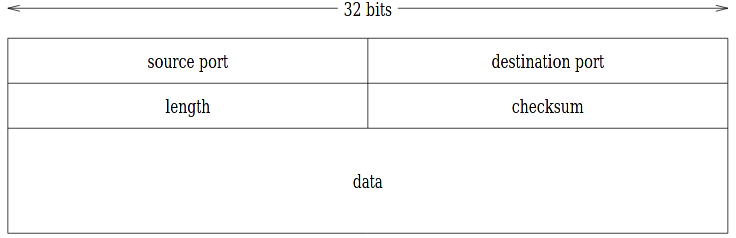
\includegraphics[width=0.7\textwidth]{udp_header}
    \caption{UDP header format \cite{udp_header}}
    \label{fig:uds_header}
\end{figure}

The UDP header format contains four header fields the payload. The header fields are translated literally into the Scapy class \textbf{UDP}. The data field is not part of it because Scapy uses an explicit operator to append data to the header information. This is shown later.

The following code snippet shows the mentioned class in the Scapy library.

\begin{samepage}
\begin{minted}{python}
class UDP(Packet):
   fields_desc = [ShortEnumField('sport', 53, UDP_SERVICES),
                  ShortEnumField('dport', 53, UDP_SERVICES),
                  ShortField('len', None),
                  XShortField('chksum', None)]
\end{minted}
\end{samepage}

As in common programmer language, \textbf{short} specifies 16 bits. Since the UDP header only contains 16 bits fields, the Scapy definition only includes \textbf{short} fields. The first parameter of a field is always the name of this field. \textbf{sport} stands for source port, and \textbf{dport} for destination port.
The next parameter sets the default value for this field. This is defined by the Scapy programmers to the best of their knowledge and not by the official UDP standard. \textbf{53} specifies the DNS protocol.
\textbf{EnumField}s also contain a third argument, a simple dictionary mapping from machine-readable values to human-readable texts. For example, part of the \textbf{UDP\_SERVICES} dictionary is: \mintinline{python}{{53: 'domain', 80: 'www_http'}}.
The difference between the ShortField and XShortField is only the representation, being displayed as a decimal hex and a hex value, respectively.

The following snippet shows some examples of how to instantiate an object of the UDP class and also demonstrates how to append data to the headers with the “/” operator.

\begin{samepage}
\begin{minted}{python}
packet = UDP(dport=80) # is equivalent to:
packet = UDP(dport='www_http')

# Append 0x00 as data
packet = UDP(dport=80) / Raw(b'\x00')
\end{minted}
\end{samepage}

Scapy provides many kinds of sockets to transmit and receive packets. For example the \textbf{L2Socket} and the \textbf{L3PacketSocket}. The difference is that L2Sockets expect a packet containing all information starting from Ethernet (layer 2), while L3PacketSockets expect a packet only containing all information starting from IP (layer 3). The following code snippet illustrates how an Ethernet packet is sent via a L2Socket (Note: Root privileges might be necessary for this to work):

\begin{samepage}
\begin{minted}{python}
# import necessary classes
from scapy.arch.linux import L2Socket
# Create a layer 2 socket specifying the interface name
socket = L2Socket('eth0')
# Create a packet covering layer 2 to 7, targeting the Google server
# This packet starts a TCP handshake, thus the SYN flag is exclusively set
# Set destination port to HTTP and a high source port
packet = Ether() / IP(dst='142.250.185.163') / TCP(flags='S', dport=80, sport=60123)
# sr1 stands for: send receive one
# it sends the given packet and returns the response
response = socket.sr1(packet)
# This displays the response in a human-friendly form
response.show()
\end{minted}
\end{samepage}

The \emph{show} method gives the following output. It has been slightly edited to be more compact and some information has been replaced by placeholders for privacy reasons.

\begin{samepage}
\begin{minted}{text}
###[ Ethernet ]### 
  dst       = 12:34:45:67:89:ab
  src       = 13:37:42:be:ef:00
  type      = IPv4
###[ IP ]### 
     version   = 4
     src       = 142.250.185.163
     dst       = 123.123.123.123
###[ TCP ]### 
        sport     = www_http
        dport     = 60123
        flags     = SA
\end{minted}
\end{samepage}

The SYN and ACK flags are now set as expected for the TCP handshake. Furthermore, the sport of the request is the dport of the response.

\subsection{UDS implementation of the Scapy library}

One of the core classes in Scapy is the \mintinline{python}{Packet} class. All definitions of network packet layers, such as Ethernet, IP, TCP, CAN, UDS and so on, are defined in a class inheriting from it.

Its most important member is the \mintinline{python}{fields_desc} list. It is a requirement for each layer to overwrite it. Its elements must inherit from the \mintinline{python}{Field} class. The chosen field classes define the structure of each header field.

\begin{samepage}
    \begin{minted}{python}
    class UDS(Packet):
        services = {
             0x10: 'DiagnosticSessionControl',
             # [...]
             0x22: 'ReadDataByIdentifier',
             # [...]
             0x7f: 'NegativeResponse'}
        fields_desc = [
            XByteEnumField('service', 0, services)
        ]
    \end{minted}
\end{samepage}

The UDS layer contains only an \mintinline{python}{XByteEnumField} field. The field class names are composed of keywords.
\begin{itemize}
    \item \textbf{X}: Represent its value as a hexadecimal value for the user.
    \item \textbf{Byte}: The field has 8-bits.
    \item \textbf{Enum}: The field expects a dictionary mapping from machine-readable values to human-readable texts.
\end{itemize}

\mintinline{python}{X} and \mintinline{python}{Enum} only affect the representation of the field. The \mintinline{python}{Byte} keyword is the only one here that defines the actual structure of the field.

This particular field are given three parameters:

\begin{itemize}
    \item \mintinline{python}{'service'}: The name of the field.
    \item \mintinline{python}{0}: The default value of the field.
    \item \mintinline{python}{services}: The dictionary mapping from machine-readable values to human-readable texts.
\end{itemize}

The Scapy implementation starts a new class whenever the subsequent fields depend on a field value of the current layer. This is the case here, since the next fields depend on the value of the \mintinline{python}{service} field. The service specific fields are defined in their own classes, for example:

\begin{samepage}
\begin{minted}{python}
class UDS_DSC(Packet):
    diagnosticSessionTypes = {
             # [...]
             0x03: 'extendedDiagnosticSession',
             # [...]
    }
    fields_desc = [
        ByteEnumField('diagnosticSessionType', 0,  diagnosticSessionTypes)
    ]
\end{minted}
\end{samepage}

So far, these are two independent classes for Scapy. It doesn't know the relationship between them. This can be changed with the \mintinline{python}{bind_layers} function.

\begin{minted}{python}
bind_layers(UDS, UDS_DSC, service=0x10)
\end{minted}

This information will be used by Scapy for building and dissecting packets.

Then, if a UDS packet is received with the value 0x10 for the \mintinline{python}{service} field, it continues dissecting this packet with the field definitions of \mintinline{python}{UDS_DSC}. And vice versa, if a \mintinline{python}{UDS_DSC} packet is stacked on a \mintinline{python}{UDS} packet for building, the UDS packets \mintinline{python}{service} field automatically is set to 0x10.

Layers are stacked with the division operator of python.

\begin{samepage}
\begin{minted}{python}
packet = UDS() / UDS_DSC(diagnosticSessionType='extendedDiagnosticSession')
bytes(packet) # prints: 0x10 0x03
\end{minted}
\end{samepage}

As can be seen, the \mintinline{python}{UDS.service} field of the packet is 0x10, although it was never explicitly set. Scapy set it because of the previous binding. And because the \mintinline{python}{UDS_DSC.diagnosticSessionType} field is an enum field, its value can be set with a more expressive text value.


\subsubsection{How to work with the ISO-TP protocol}

The can-utils tools also contain applications to handle ISO-TP communication. Since this is never used in this work, but the Scapy implementation is, only the Scapy implementation is explained.

As for the CAN implementation, there are two ISO-TP socket implementations in Scapy. A software and a native implementation. Until including Linux kernel 5.9, the corresponding ISO-TP module for Linux had to be installed separately \cite{isotp-module}. Since Linux kernel 5.10, it is part of the Linux mainline kernel \cite{isotp-commit}. Both implementations handle the ISO-TP metadata themselves, i.e.  fragmentation, defragmentation, etc.

An ISO-TP socket contains a source and destination identifier. They offer the same functionality as the ports for TCP or UDP. The source identifier is the identifier of outgoing CAN packets, and the destination identifier is the identifier expected for incoming packets.

The usage of the native implementation is illustrated in the following code snippet:

\begin{samepage}
\begin{minted}{python}
from scapy.contrib.isotp import ISOTPNativeSocket
socket = ISOTPNativeSocket('vcan0', sid=0x123, did=0x456)
packet = Raw(b'\x01\x02')
socket.send(packet)
\end{minted}
\end{samepage}

\subsection{Explaining the service enumerators of the UDS Scanner}

% TODO: Add that it was still work in progress while doing this work
% and thus, that problems occured and had to be fixed.
% Out of scope of this work.

Enumerators are service-specific and create all possible requests for a service.
For example, the enumerator for the DSC service is called UDS\_DSCEnumerator. The most important member of the enumerator classes is the \mintinline{python}{_get_initial_requests} method. The return value is an iterable object which contains all requests for this service. DSC has an eight bit identifier, leading to a maximum of 2\textsuperscript{8} packets for this service. Each enumerator will be executed for each found state of the ECU. So, if an enumerator already ran, and afterwards a new state is found, this enumerator will run again within the same scan with the new-found state.

For a better understanding, the UDS\_DSCEnumerator implementation will be described exemplary.

\begin{samepage}
\begin{minted}{python}
class UDS_DSCEnumerator(UDS_Enumerator, StateGenerator):
    def _get_initial_requests(self, **kwargs):
        session_range = kwargs.pop('session_range', range(2, 0x100))
        return UDS() / UDS_DSC(diagnosticSessionType=session_range)
\end{minted}
\end{samepage}

The method can be given keyword parameters. The only one used here is \mintinline{python}{session_range}. If none is given, which is usually the case, it defaults to the range from 0x02 to 0xff. So, this enumerator creates 254 packets for each state. This service is a StateGenerator, which means its requests can change the state of the ECU. This is detected by the UDS Scanner and the new state will be scanned as well.

So-called staged enumerators contain enumerators where each enumerator is a stage. They start executing the first enumerator for each state, followed by each subsequent enumerator in the same way. For each stage transition (for example $1 \rightarrow 2$ or $2 \rightarrow 3$) connectors can be defined. They are functions with two arguments, containing the previous enumerator and the new enumerator. Here the results of the previous enumerator can be evaluated and the new enumerator can be configured accordingly.

Enumerators can output their results as a text-table. For example:

\begin{samepage}
\begin{minted}{text}
---------------+---------------+---------------+---------------+
               | session1      | session1tp1   | session3tp1   | 
---------------+---------------+---------------+---------------+
TesterPresent: | PR: Supported | PR: Supported | PR: Supported | 
---------------+---------------+---------------+---------------+
\end{minted}
\end{samepage}

This means, the request of the TesterPresent service was positively answered by the ECU in all three found states.

\subsection{Implementing new enumerators for the RC service}

Three classes are of interest:

\begin{itemize}
    \item \textbf{RCEnumerator}: Defaults to scanning the whole RC service, including all three types.
    \item \textbf{RCStartEnumerator}: Only scanning Type1 of the RC service.
    \item \textbf{RCSelectiveEnumerator}: Staged enumerator containing an RCStartEnumerator and an RCEnumerator.
\end{itemize}

\begin{figure}[h]
    \centering
    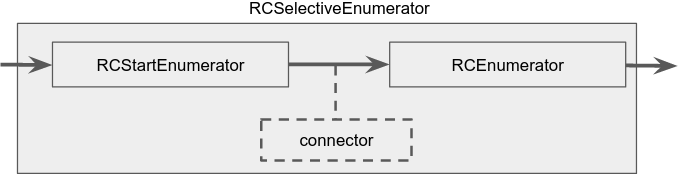
\includegraphics[width=0.7\textwidth]{rc-schematic}
    \caption{Schematic illustration of the new RCSelectiveEnumerator.}
    \label{fig:rc-schematic}
\end{figure}

The connector of the RCSelectiveEnumerator expands the found identifiers of the RCStartEnumerator to ranges and also resolves any overlaps to a continuous range and forwards these ranges to the second stage, the RCEnumerator. Additionally, the connector configures the RCEnumerator to only scan Type2 and Type3.

Each positively answered identifier of Type1 in any state will also be probed for all subsequent states in Type2 and Type3, even if this identifier is not found in Type1 for another state. This increases the coverage in cases, where a routine can be started in a state, but its result, or to stop it, may only be requested in another state.

\begin{minted}{python}
    class UDS_RCEnumerator(UDS_Enumerator):
        _description = "Available RoutineControls and negative response per state"
    
        def _get_initial_requests(self, **kwargs):
            # type: (Any) -> Iterable[Packet]
            type_list = kwargs.pop("type_list", [1, 2, 3])
            scan_range = kwargs.pop("scan_range", range(0x10000))
    
            return (
                UDS() / UDS_RC(routineControlType=rc_type,
                               routineIdentifier=data_id)
                for rc_type, data_id in itertools.product(type_list, scan_range)
            )
    
        @staticmethod
        def _get_table_entry(tup):
            # type: (_AutomotiveTestCaseScanResult) -> Tuple[EcuState, str, str]
            state, req, res, _, _ = tup
            label = UDS_Enumerator._get_label(res)
            return (state,
                    "0x%04x-%d: %s" % (
                        req.routineIdentifier, req.routineControlType,
                        req.sprintf("%UDS_RC.routineIdentifier%")),
                    label)
\end{minted}

    
\begin{minted}{python}
    class UDS_RCStartEnumerator(UDS_RCEnumerator):
        _description = "Available RoutineControls and negative response per state"
    
        def _get_initial_requests(self, **kwargs):
            # type: (Any) -> Iterable[Packet]
            if "type_list" in kwargs:
                raise KeyError("'type_list' already set in kwargs.")
            kwargs["type_list"] = [1]
            return super(UDS_RCStartEnumerator, self). \
                _get_initial_requests(**kwargs)
\end{minted}

\begin{minted}{python}
    class UDS_RCSelectiveEnumerator(StagedAutomotiveTestCase):
        # Used to expand points to both sites
        # So, the total block size will be 253 * 2 = 506
        expansion_width = 253
    
        @staticmethod
        def points_to_ranges(pois):
            # type: (Iterable[int]) -> Iterable[int]
            expansion_width = UDS_RCSelectiveEnumerator.expansion_width
            generators = []
            for identifier in pois:
                start = max(identifier - expansion_width, 0)
                end = min(identifier + expansion_width + 1, 0x10000)
                generators.append(range(start, end))
            ranges_with_overlaps = itertools.chain.from_iterable(generators)
            return sorted(set(ranges_with_overlaps))
    
        @staticmethod
        def __connector_start_to_rest(rc_start, _rc_stop):
            # type: (AutomotiveTestCaseABC, AutomotiveTestCaseABC) -> Dict[str, Any]  # noqa: E501
            rc_start = cast(UDS_Enumerator, rc_start)
            identifiers_with_pr = [resp.routineIdentifier for _, _, resp, _, _
                                   in rc_start.results_with_positive_response]
            scan_range = UDS_RCSelectiveEnumerator.points_to_ranges(
                identifiers_with_pr)
    
            return {"type_list": [2, 3],
                    "scan_range": scan_range}
    
        def __init__(self):
            # type: () -> None
            super(UDS_RCSelectiveEnumerator, self).__init__(
                [UDS_RCStartEnumerator(), UDS_RCEnumerator()],
                [None, self.__connector_start_to_rest])
    
\end{minted}

\subsection{Implementing new enumerators for the RDBI service}

Again, three classes are of interest:

\begin{itemize}
    \item \textbf{RDBIEnumerator}: Defaults to scanning the whole RDBI service.
    \item \textbf{RDBIRandomEnumerator}: Scanning block-based with random identifiers.
    \item \textbf{RDBISelectiveEnumerator}: Staged enumerator containing an RDBIRandomEnumerator and an RDBIEnumerator.
\end{itemize}

\begin{figure}[h]
    \centering
    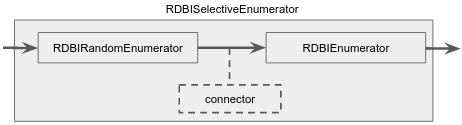
\includegraphics[width=0.7\textwidth]{rdbi-schematic}
    \caption{Schematic illustration of the new RDBISelectiveEnumerator.}
    \label{fig:rdbi-schematic}
\end{figure}

Similar to the previous approach, the new implementation is two-staged. First, the RDBIRandomEnumerator is executed. Then, the connector creates requests for whole blocks, if any of their requests were answered positively, and ensured that for a single block each identifier is queried only once. The resulting packets are passed to the configurable RDBIEnumerator.

Also, as with the RCSelectiveEnumerator, each positively answered identifier will be remembered for all subsequent states. This increases the coverage because most identifiers are also available in other states, but the RandomEnumerator might not detect them for each state.

Implementing the RDBIRandomEnumerator was a challenge because it must include the probabilities of occurence of positively responded identifiers for each block. With a block size of $2^6$, there would need to be a list with $\frac{2^{16}}{2^6} = 1024$ elements. Thus, it is desirable to represent this information more compactly. A better representation is based on two facts. That the probabilities are ultimately calculated to the number of samples, and that at least one request should be generated for each block. For the former, the number of samples for each block were pre-computed instead of being computed at runtime. This simplifies the list in the sense that integers are stored instead of float values. Second, the number of samples is not stored for all blocks, but only for blocks whose number of samples is greater than or equal to 2. And blocks for which no value is stored, the value 1 is used. This automatically solves that each block is probed with at least one packet, even if its probability is 0\%. These simplifications transformed the list of 1024 elements into a dictionary of only 109 elements.

\begin{minted}{python}
    class UDS_RDBIEnumerator(UDS_Enumerator):
        _description = "Readable data identifier per state"

        def _get_initial_requests(self, **kwargs):
            # type: (Any) -> Iterable[Packet]
            scan_range = kwargs.pop("scan_range", range(0x10000))
            return (UDS() / UDS_RDBI(identifiers=[x]) for x in scan_range)
\end{minted}
    
\begin{minted}{python}
    class UDS_RDBISelectiveEnumerator(StagedAutomotiveTestCase):
        @staticmethod
        def __connector_random_to_sequential(rdbi_random, _):
            # type: (UDS_RDBIRandomEnumerator, UDS_RDBIEnumerator) -> Dict[str, Any]
            rdbi_random = cast(UDS_Enumerator, rdbi_random)
            identifiers_with_positive_response = \
                [p.resp.dataIdentifier
                 for p in rdbi_random.results_with_positive_response]
    
            scan_range = UDS_RDBISelectiveEnumerator. \
                points_to_blocks(identifiers_with_positive_response)
            return {"scan_range": scan_range}
    
        @staticmethod
        def points_to_blocks(pois):
            # type: (Sequence[int]) -> Iterable[int]
            block_size = UDS_RDBIRandomEnumerator.block_size
            generators = []
            for start in range(0, 2 ** 16, block_size):
                end = start + block_size
                pr_in_block = any((start <= identifier < end
                                   for identifier in pois))
                if pr_in_block:
                    generators.append(range(start, end))
            scan_range = itertools.chain.from_iterable(generators)
            return scan_range
    
        def __init__(self):
            # type: () -> None
            super(UDS_RDBISelectiveEnumerator, self).__init__(
                [UDS_RDBIRandomEnumerator(), UDS_RDBIEnumerator()],
                [None, self.__connector_random_to_sequential])
\end{minted}

\begin{minted}{python}
    class UDS_RDBIRandomEnumerator(UDS_RDBIEnumerator):
        block_size = 2 ** 6
    
        def _get_initial_requests(self, **kwargs):
            # type: (Any) -> Iterable[Packet]
    
            samples_per_block = {
                4: 29, 5: 22, 6: 19, 8: 11, 9: 11, 10: 13, 11: 14, 12: 31, 13: 4,
                14: 26, 16: 30, 17: 4, 18: 20, 19: 5, 20: 49, 21: 54, 22: 9, 23: 4,
                24: 10, 25: 8, 28: 6, 29: 3, 32: 11, 36: 4, 37: 3, 40: 9, 41: 9,
                42: 3, 44: 2, 47: 3, 48: 4, 49: 3, 52: 8, 64: 35, 66: 2, 68: 24,
                69: 19, 70: 30, 71: 28, 72: 16, 73: 4, 74: 6, 75: 27, 76: 41,
                77: 11, 78: 6, 81: 2, 88: 3, 90: 2, 92: 16, 97: 15, 98: 20, 100: 6,
                101: 5, 102: 5, 103: 10, 106: 10, 108: 4, 124: 3, 128: 7, 136: 15,
                137: 14, 138: 27, 139: 10, 148: 9, 150: 2, 152: 2, 168: 23,
                169: 15, 170: 16, 171: 16, 172: 2, 176: 3, 177: 4, 178: 2, 187: 2,
                232: 3, 235: 2, 240: 8, 252: 25, 256: 7, 257: 2, 287: 6, 290: 2,
                316: 2, 319: 3, 323: 3, 324: 19, 326: 2, 327: 2, 330: 4, 331: 10,
                332: 3, 334: 8, 338: 3, 832: 6, 833: 2, 900: 4, 956: 4, 958: 3,
                964: 12, 965: 13, 966: 34, 967: 3, 972: 10, 1000: 3, 1012: 23,
                1013: 14, 1014: 15
            }
            to_scan = []
            block_size = UDS_RDBIRandomEnumerator.block_size
            for block_index, start in enumerate(range(0, 2 ** 16, block_size)):
                end = start + block_size
                count_samples = samples_per_block.get(block_index, 1)
                to_scan += random.sample(range(start, end), count_samples)
    
            # Use locality effect
            # If an identifier brought a positive response in any state,
            # it is likely that in another state it is available as well
            positive_identifiers = [t.resp.dataIdentifier for t in
                                    self.results_with_positive_response]
            to_scan += positive_identifiers
    
            # make all identifiers unique with set()
            # Sort for better logs
            to_scan = sorted(list(set(to_scan)))
            return (UDS() / UDS_RDBI(identifiers=[x]) for x in to_scan)
\end{minted}

The non-compact version is shown in \autoref{app:random-not-compact}.

\subsection{Extending the UDS Scanner to skip unsupported services}

In contrast to the previous approaches, this one is not applied to an enumerator, but to the UDS Scanner itself. The UDS Scanner evaluates each response, for example to detect if a new state was found. Here, a check was added for negative responses if they have the NRC 0x11 or 0x7f. If they do, the enumerator is set to completed for the currently executed state. This behavior has to be enabled explicitly, because as the next section explains, it might result in losses.

\begin{minted}{python}
    class AutomotiveTestCase(AutomotiveTestCaseABC):
        """Base class for Enumerators"""
    
        def _evaluate_response(self, response, **kwargs):
            # type: (Optional[Packet], Optional[Dict[str, Any]]) -> bool
    
            # Removed code for simplification
    
            exit_if_service_not_supported = kwargs.pop(
                "exit_if_service_not_supported", False)
    
            if exit_if_service_not_supported and response.service == 0x7f:
                response_code = self._get_negative_response_code(response)
                if response_code in [0x11, 0x7f]:
                    names = {0x11: "serviceNotSupported",
                                0x7f: "serviceNotSupportedInActiveSession"}
                    msg = "[-] Exit execute because negative response " \
                            "%s received!" % names[response_code]
                    log_interactive.debug(msg)
                    # execute of current state is completed,
                    # since a serviceNotSupported negative response was received
                    self._state_completed[self._results[-1].state] = True
                    # stop current execute and exit
                    return True
    
            # Removed code for simplification
    
            return False
\end{minted}
    
